\chapter{ANALISIS DAN PERANCANGAN SISTEM} \label{chap:analisis-perancangan-sistem}
\tab Pada bab ini akan dijelaskan mengenai analisis dan perancangan sistem perangkat lunak yang akan dibangun, meliputi struktur data, algoritme, dan arsitektur aplikasi. 

\section{Daftar Notasi}
\tab Tabel \ref{tab:daftar-notasi-2} menunjukkan daftar notasi yang digunakan dalam bab ini beserta deskripsinya.

\begin{longtable}{| p{3cm} | p{6cm} |} 
	\caption{Daftar Notasi (2) \label{tab:daftar-notasi-2}}\\
	\hline
	\textbf{Notasi} & \textbf{Deskripsi}\\ \hline
	\endfirsthead
	\hline
	\textbf{Notasi} & \textbf{Deskripsi}\\ \hline
	\endhead
	$P$ & \textit{Dataset} produk\\ \hline
	$C$ & \textit{Dataset} pelanggan (preferensi pelanggan)\\ \hline
	$D$ & $P \cup C$ \\ \hline
	$E$ & Himpunan \textit{event} \\ \hline
	$p$ & Sebuah produk dalam $P$, $p \in P$\\ \hline
	$c$ & Seorang pelanggan dalam $C$, $c \in C$\\ \hline
	$e$ & Sebuah \textit{event} dalam $E$, $e \in E$ \\ \hline
	$p_{in}$ & Produk masuk \\ \hline
	$p_{out}$ & Produk keluar \\ \hline
	$c_{in}$ & Pelanggan masuk \\ \hline
	$c_{out}$ & Pelanggan keluar \\ \hline
	$P_{active}$ & Himpunan produk yang sedang aktif (di dalam lini masa) \\ \hline	
	$C_{active}$ & Himpunan pelanggan yang sedang aktif (di dalam lini masa) \\ \hline	
	$D_{active}$ & $P_{active} \cup C_{active}$ \\ \hline	
	$d$ & Jumlah dimensi pada $D$\\ \hline
	$i$ & Dimensi ke-1, ..., $d$\\ \hline
	$j$ & Timestamp ke-1, 2, ..., dst\\ \hline
	$diff$ & Selisih nilai \\ \hline
	$p_s$ & Produk sebagai subjek yang membandingkan \\ \hline
	$p_o$ & Produk sebagai objek pembanding \\ \hline
	$O$ & \textit{Orthant}\\ \hline
	$pos_x(p)$ & Posisi $p$ pada sumbu $x$ \\ \hline
	$max_x$ & Nilai maksimum pada sumbu $x$ \\ \hline
	$m$ & \textit{Midpoint} antar produk\\ \hline
	$DSL(c)$ & Hasil \textit{dynamic skyline} dari pelanggan $c$\\ \hline
	$RSL(p)$ & Hasil \textit{reverse skyline} dari produk $p$\\ \hline
	$Pr(c, p|P)$ & Probabilitas produk $p$ dibeli oleh pelanggan $c$ \\ \hline
	$E(C, p|P)$ & Kontribusi pasar $p$\\ \hline
	$E(C, P'|P)$ & Kontribusi pasar subset $P'$ dari $P$ \\ \hline
	$k-MPPTI$ & \textit{k-Most Promising Products in Time Intervals} \\ \hline
	$k$ & Jumlah data \\ \hline
	$[t_i:t_e]$ & Interval waktu \\ \hline
	$PBox$ & \textit{Pandora Box} \\ \hline	
	$ts$ & \textit{Timestamp} \\ \hline	
\end{longtable}

\section{Analisis Sistem}
\tab Analisis sistem dijelaskan dalam empat bagian, yakni analisis permasalahan, deskripsi umum sistem, fungsi sistem, dan analisis kebutuhan fungsional.

\subsection{Analisis Permasalahan}
\tab Permalasahan yang ingin diselesaikan pada Tugas Akhir ini adalah bagaimana menjawab kueri \textit{$k$-Most Promising Products} berbasis interval waktu ($k$-MPPTI). Interval waktu, dinotasikan dengan $[t_i:t_e ](t_i \leq t_e)$, digunakan untuk menentukan rentang waktu pencarian.

Permasalahan ini tidak dapat langsung diselesaikan menggunakan metode dan algoritme yang sudah ada \cite{kmpp}. Sehingga, diperlukan pendekatan lain yang akan dijelaskan pada bagian perancangan sistem.

\subsection{Deskripsi Umum Sistem}
\tab Secara umum, sistem yang akan dibangun adalah sebuah sistem berbasis web yang dapat membantu pengguna untuk memilih \textit{k}-produk yang paling menjanjikan. Dikatakan "menjanjikan" jika produk tersebut memiliki kontribusi pasar yang besar.

Sistem ini memiliki dua proses utama, yaitu (1) \textit{data precomputing} untuk menghitung kontribusi pasar masing-masing produk dan (2) proses utama (selanjutnya akan disebut dengan \textit{query processing}) untuk memproses dan menampilkan hasil kueri pencarian yang dimasukkan oleh pengguna.

Sistem ini dibangun menggunakan arsitektur \textit{client}-\textit{server}. Aplikasi \textit{client} didesain berbasis web dengan memanfaatkan Flask \textit{microframework}, HTML, CSS, dan JavaScript. Selain itu, Flask juga digunakan sebagai \textit{web server}. 

\subsection{Fungsi Sistem}
\tab Sistem yang akan dibangun memiliki beberapa fungsi utama sebagai berikut:
\begin{enumerate}
	\item Dapat menerima masukan data berupa file dari pengguna
	\item Dapat menampilkan informasi dan pratinjau data yang dimasukkan oleh pengguna
	\item Dapat menampilkan visualisasi data
	\item Dapat melakukan proses \textit{data precomputing} menggunakan algoritme yang dipilih oleh pengguna
	\item Dapat menerima masukan kueri pencarian 
	\item Dapat memproses kueri pencarian
	\item Dapat menampilkan hasil kueri
	\item Dapat menampilkan waktu eksekusi
\end{enumerate}

\subsection{Analisis Kebutuhan Fungsional}
\tab Sistem yang dibuat harus mampu memenuhi beberapa fungsi utama yang telah dijelaskan pada sub-bagian sebelumnya. Fungsi-fungsi ini merupakan hasil dari analisis kebutuhan fungsional dari pengguna yang dijelaskan pada Tabel \ref{tab:kebutuhan-fungsional}.

\begin{table}[H]
	\centering
	\begin{tabular}{ | p{2cm} | p{7cm} | }
		\hline
		\textbf{Kode} & \textbf{Deskripsi Kebutuhan} \\ \hline \hline
		F-001 & Mengunggah data \\ \hline
		F-002 & Melihat informasi dan pratinjau data \\ \hline
		F-003 & Melihat visualisasi data  \\ \hline
		F-004 & Memilih algoritme yang digunakan untuk \textit{data precomputing}\\ \hline
		F-005 & Memasukkan kueri pencarian \\ \hline
		F-006 & Melihat hasil kueri \\ \hline
		F-007 & Melihat waktu eksekusi \\ \hline
	\end{tabular} \caption{Kebutuhan Fungsional}
	\label{tab:kebutuhan-fungsional}
\end{table}

Penjelasan rinci dari masing-masing kebutuhan fungsional pada tabel \ref{tab:kebutuhan-fungsional} dijelaskan sebagai berikut:
\begin{enumerate}
	\item Mengunggah data\\
	Pengguna dapat mengunggah data produk dan preferensi pelanggan dalam bentuk file berekstensi csv.
	\item Melihat informasi dan pratinjau data \\
	Pengguna dapat melihat informasi dan pratinjau dari data yang dimasukkan berupa tabel sebanyak dua puluh baris. Informasi yang ditampilkan antara lain jumlah baris, jumlah kolom, dan nama kolom.
	\item Melihat visualisasi data \\
	Pengguna juga dapat melihat visualisasi dari data yang dimasukkan berupa lini masa sederhana.
	\item Memilih algoritme yang digunakan untuk \textit{data precomputing} \\
	Pengguna dapat memilih algoritme yang akan digunakan untuk \textit{data precomputing}, yaitu algoritme $k$-MPPTI dan \textit{Brute Force}.
	\item Memasukkan kueri pencarian \\
	Pengguna dapat memasukkan kueri pencarian berupa jumlah produk ($k$) dan interval waktu.
	\item Melihat hasil kueri \\
	Pengguna dapat melihat hasil kueri pencarian berupa $k$-produk dengan jumlah kontribusi pasar terbesar beserta skor kontribusi pasar-nya. 
	\item Melihat waktu eksekusi \\
	Pengguna dapat melihat informasi terkait waktu eksekusi.
\end{enumerate}

\section{Perancangan Sistem}
\tab Perancangan sistem akan dibagi menjadi empat bagian, yakni struktur data, algoritme utama, algoritme pembanding menggunakan metode \textit{brute force}, dan arsitektur aplikasi. 

\subsection{Struktur Data}
\tab Struktur data adalah suatu cara untuk menyimpan, menyusun, mengelompokkan, dan merepresentasikan suatu data. Ada tiga struktur data utama yang digunakan dalam komputasi $k$-MPPTI, yaitu \textit{Data Storage}, \textit{Event Queue}, dan \textit{Pandora Box}.

\subsubsection{\textit{Data Storage}}
\tab \textit{Data Storage} adalah sebuah struktur data \textit{dictionary} yang digunakan untuk menyimpan data produk dan pelanggan. Struktur data \textit{dictionary} lebih efisien untuk pencarian data karena menggunakan konsep \textit{key-value pairs}, berbeda dengan struktur data \textit{list} atau \textit{array} yang menggunakan indeks untuk mengakses nilai suatu data.

\begin{figure}[H]
	\centering
	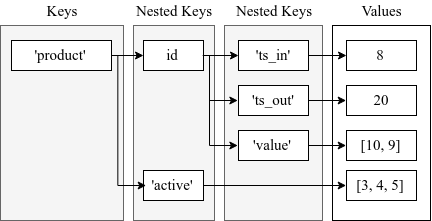
\includegraphics[width=7cm]{assets/img/bab3/sd1.png}
	\caption{Struktur Data \textit{Dictionary} Produk}
	\label{fig:sd1}
\end{figure}

\begin{figure}[H]
	\centering
	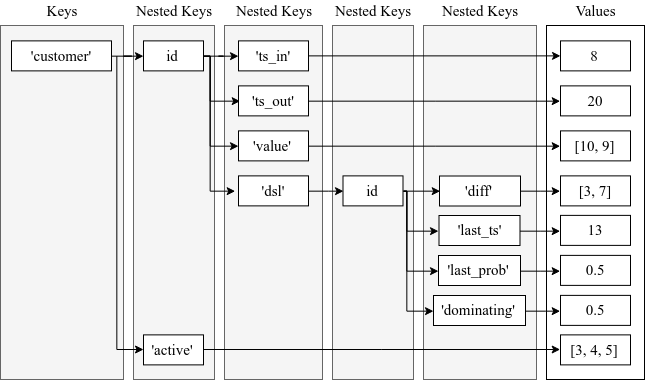
\includegraphics[width=9cm]{assets/img/bab3/sd2.png}
	\caption{Struktur Data \textit{Dictionary} Pelanggan}
	\label{fig:sd2}
\end{figure}

Struktur data \textit{dictionary} yang digunakan berbentuk \textit{nested dictionary} yang terdiri dari dua \textit{key} utama, yaitu '$product$' yang menyimpan data produk dan '$customer$' yang menyimpan data pelanggan. Struktur \textit{nested key} masing-masing data dijelaskan pada Gambar \ref{fig:sd1} dan \ref{fig:sd2} dan deskripsinya dijelaskan pada Tabel \ref{tab:desc-key}.

\begin{longtable}{| p{2.5cm} | p{6.5cm} |}
	\caption{\textit{Key} dari \textit{Data Storage} \label{tab:desc-key}}\\
	\hline
	\textbf{\textit{Key}} & \textbf{Deskripsi} \\ \hline 
	\endfirsthead
	\hline
	\textbf{\textit{Key}} & \textbf{Deskripsi} \\ \hline 
	\endhead
	$'product'$ & Menyimpan data produk \\ \hline
	$'customer'$ & Menyimpan data pelanggan \\ \hline
	$id$ & ID data produk atau pelanggan dijadikan sebagai \textit{key} \\ \hline
	$'active'$ & Menyimpan ID data produk atau pelanggan yang sedang aktif dalam bentuk \textit{array} \\ \hline
	$'ts\_in'$ & Menyimpan \textit{timestamp} atau waktu masuk \\ \hline
	$'ts\_out'$ & Menyimpan \textit{timestamp} atau waktu keluar \\ \hline
	$'value'$ & Menyimpan nilai data produk atau pelanggan pada semua dimensi dalam bentuk \textit{array}\\ \hline
	$'dsl'$ & Menyimpan hasil \textit{dynamic skyline} dalam bentuk \textit{dictionary} dengan $id$ produk sebagai \textit{key}\\ \hline
	$'diff'$ & Menyimpan selisih antara nilai data produk dan pelanggan pada masing-masing dimensi \\ \hline
	$'last\_ts'$ & Menyimpan \textit{timestamp} terakhir saat diperbarui ke \textit{Pandora Box}\\ \hline
	$'last\_prob'$ & Menyimpan probabilitas terakhir saat diperbarui ke \textit{Pandora Box}\\ \hline
	$'dominating'$ & Menyimpan ID produk lain yang pernah didominasi\\ \hline
\end{longtable}

\subsubsection{\textit{Event Queue}}
\tab \textit{Event} adalah titik-titik tempat terjadinya perubahan di dalam himpunan data, yaitu jika ada data yang masuk atau keluar. Ada empat jenis \textit{event} yang terjadi dalam penelitian ini, yaitu:

\begin{enumerate}
	\item Data Produk masuk
	\item Data Produk keluar
	\item Data Pelanggan masuk
	\item Data Pelanggan keluar
\end{enumerate}
Produk dan pelanggan disebut dengan pemilik \textit{event}, sedangkan masuk dan keluar disebut dengan aksi \textit{event}.

\textit{Event Queue} adalah sebuah struktur data \textit{queue} yang berfungsi untuk menyimpan \textit{event-event} yang terjadi di dalam himpunan data. \textit{Queue} memiliki prinsip FIFO (\textit{First In First Out}), sehingga \textit{event} akan diproses secara berurutan menurut antrian waktu. \textit{Event Queue} menyimpan empat informasi, yaitu \textit{timestamp}, pemilik \textit{event}, ID pemilik \textit{event}, dan aksi \textit{event}. Untuk lebih jelasnya, atribut \textit{Event Queue} dijelaskan pada Tabel \ref{tab:attr-event-queue}.


\begin{table}[H]
	\centering
	\begin{tabular}{|p{2cm}|p{6cm}|}
		\hline
		\textbf{Atribut} & \textbf{Deskripsi} \\ \hline \hline
		$timestamp$ & Waktu terjadinya \textit{event} \\ \hline
		$owner$ & Pemilik \textit{event} (produk $= 0$, pelanggan $= 1$) \\ \hline
		$ownerId$ & ID pemilik \textit{event}\\ \hline
		$action$ & Jenis aksi yang dilakukan (masuk $= 0$, keluar $= 1$) \\ \hline
	\end{tabular} 
	\caption{Atribut dari \textit{Event Queue}}
	\label{tab:attr-event-queue}
\end{table}

\subsubsection{\textit{Pandora Box}}
\tab \textit{Pandora Box} adalah sebuah struktur data \textit{array} dua dimensi yang terdiri dari sumbu $x$ (\textit{time series}) dan sumbu $y$ (produk). Struktur data ini digunakan untuk menyimpan skor kontribusi pasar produk setiap waktu. Menggunakan contoh \textit{dataset} pada Tabel \ref{tab:dataset-2}, maka model \textit{Pandora Box} yang terbentuk adalah seperti pada Gambar \ref{fig:pbox}.  

\begin{figure}[h]
	\centering
	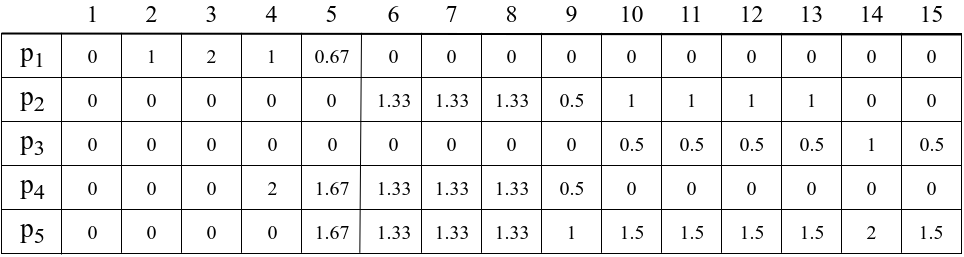
\includegraphics[width=10cm]{assets/img/bab3/pbox.png}
	\caption{Contoh \textit{Pandora Box} dari \textit{Dataset} \ref{tab:dataset-2}}
	\label{fig:pbox}
\end{figure}

\subsection{Algoritme Utama}
\tab Sebagaimana yang telah dijelaskan sebelumnya bahwa algoritme $k$-MPPTI terdiri dari dua tahap pemrosesan, yaitu \textit{data precomputing} dan \textit{query processing}. Secara garis besar, alur kerja sistem secara umum disajikan dalam bentuk diagram alur yang dapat dilihat pada Gambar \ref{fig:diagram-alur1}.

\begin{figure}[H]
	\centering
	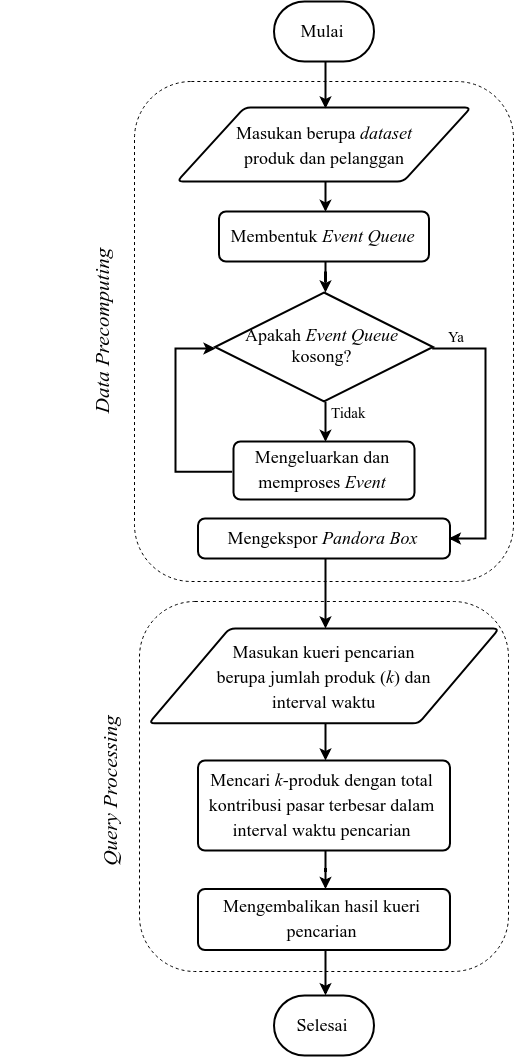
\includegraphics[width=10cm]{assets/img/bab3/flowchart.png}
	\caption{Diagram Alur Algoritme k-MPPTI}
	\label{fig:diagram-alur1}
\end{figure}

Tahap \textit{data precomputing} bertujuan untuk menghitung skor kontribusi pasar masing-masing produk berdasarkan preferensi pelanggan. Diawali dengan pembentukan \textit{Event Queue} untuk mencatat semua \textit{event} yang terjadi selama pemrosesan data. Kemudian, memproses \textit{event-event} tersebut menggunakan algoritme pemrosesan berdasarkan jenis \textit{event}-nya. Terakhir adalah mengekspor \textit{Pandora Box} untuk digunakan sebagai masukan pada tahap \textit{query processing}.

Tahap kedua adalah \textit{query processing} yang bertujuan untuk memproses kueri pencarian yang dimasukkan oleh pengguna berupa jumlah produk ($k$) dan interval waktu pencarian. Diawali dengan mencari produk sejumlah $k$ yang memiliki total skor kontribusi pasar terbesar selama interval waktu pencarian, kemudian mengembalikan hasil kueri pencarian berupa $k$-produk yang paling menjanjikan kepada pengguna.

Untuk memudahkan interaksi antara pengguna dan sistem, dibuatlah aplikasi berbasis web yang memudahkan pengguna memasukkan data produk dan pelanggan, melihat pratinjau dan visualisasi data, memasukkan kueri pencarian, serta melihat hasil kueri pencarian.   

\subsubsection{\textit{Data Precomputing}}
\tab \textit{Data precomputing} adalah sebuah proses yang dapat menunjang performa algoritme \textit{query processing} supaya dapat bekerja lebih efektif dan efisien. Tidak adanya proses \textit{data precomputing} menyebabkan pengulangan komputasi data setiap kali seseorang memasukkan kueri pencarian. Karena data yang digunakan adalah \textit{historical data}, yaitu data yang dikumpulkan dari kejadian yang telah lalu, maka komputasi data cukup dilakukan satu kali saja di awal (\textit{precomputing}). Berbeda halnya jika data yang digunakan adalah \textit{streaming data} yang nilainya terus berubah dalam periode waktu tertentu.
	
\newcolumntype{C}{>{\centering\arraybackslash}p{1.4em}}
\begin{table}[H]
	\caption{Contoh \textit{Dataset} \\ (a) Produk $P$ dan (b) Preferensi Pelanggan $C$ \label{tab:dataset-2}}
	\begin{subtable}{.5\linewidth}
		\small
		\centering
		\caption{}
		\begin{tabular}{|C|C|C|C|C|}
			\hline
			\multirow{2}{*}{\textbf{ID}} & \multicolumn{2}{c|}{\textbf{\textit{Timestamp}}} & \multicolumn{2}{c|}{\textbf{Nilai}} \\ \cline{2-5}
			& \textbf{$t_i$} & \textbf{$t_e$} & \textbf{$d_1$} & \textbf{$d_2$}\\ \hline \hline
			$p_1$ & 2 & 10 & 6 & 3 \\ \hline
			$p_2$ & 6 & 13 & 4 & 12 \\ \hline
			$p_3$ & 9 & 15 & 6 & 15 \\ \hline
			$p_4$ & 4 & 9 & 9 & 5 \\ \hline
			$p_5$ & 5 & 15 & 12 & 10 \\ \hline
		\end{tabular}
	\end{subtable}%
	\begin{subtable}{.5\linewidth}
		\small
		\centering
		\caption{}
		\begin{tabular}{|C|C|C|C|C|}
			\hline
			\multirow{2}{*}{\textbf{ID}} & \multicolumn{2}{c|}{\textbf{\textit{Timestamp}}} & \multicolumn{2}{c|}{\textbf{Nilai}} \\ \cline{2-5}
			 & \textbf{$t_i$} & \textbf{$t_e$} & \textbf{$d_1$} & \textbf{$d_2$}\\ \hline \hline
			$c_1$ & 1 & 8 & 2 & 8 \\ \hline
			$c_2$ & 4 & 14 & 4 & 10\\ \hline
			$c_3$ & 10 & 15 & 6 & 11\\ \hline
			$c_4$ & 3 & 8 & 8 & 12\\ \hline
			$c_5$ & 5 & 15 & 9 & 10\\ \hline
		\end{tabular}
	\end{subtable} 
\end{table}

Pada Tabel \ref{tab:dataset-2}, diberikan contoh \textit{dataset} produk $P$ dan preferensi pelanggan $C$ yang setiap datanya direpresentasikan sebagai titik $d$-dimensi dengan serial waktu $[t_i:t_e]$. Pendekatan yang digunakan untuk memproses data multidimensi dengan serial waktu adalah menggunakan lini masa yang diilustrasikan pada Gambar \ref{fig:timeline}.
\begin{figure}[H]
	\centering
	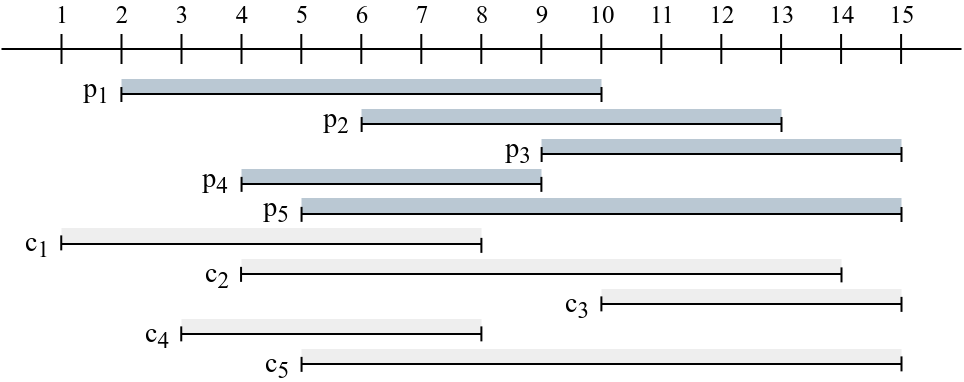
\includegraphics[width=10cm]{assets/img/bab3/timeline-polos.png}
	\caption{lini Masa Data Produk dan Pelanggan}
	\label{fig:timeline}
\end{figure}

Lini masa atau alur waktu adalah suatu representasi kronologis urutan peristiwa atau kejadian (\textit{event}). Lini masa dapat dibuat menurut era, abad, tahun, bulan, minggu, atau hari, namun untuk pemodelan ini, waktu direpresentasikan sebagai bilangan bulat positif. Di dalam lini masa, terdapat titik-titik yang mewakili kejadian penting (\textit{event}) yang dinotasikan dengan $e \in E$. 
\begin{figure}[H]
	\centering
	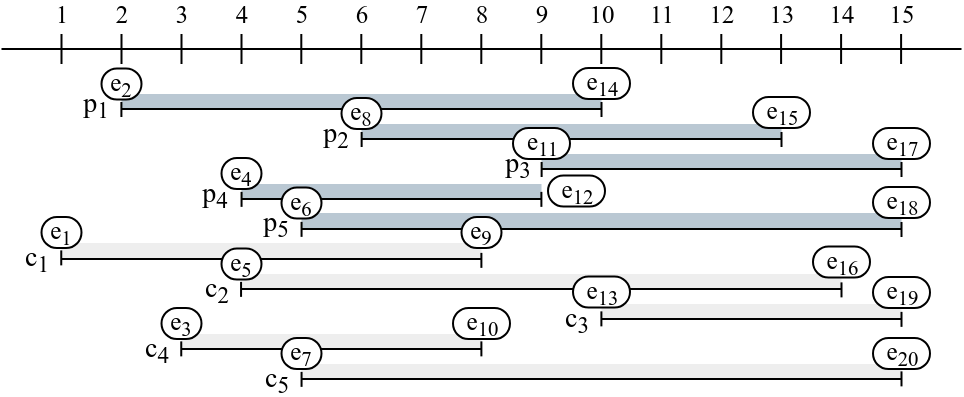
\includegraphics[width=10cm]{assets/img/bab3/timeline-event.png}
	\caption{\textit{Event} dalam Lini Masa Data Produk dan Pelanggan}
	\label{fig:timeline-event}
\end{figure}

Ada empat jenis \textit{event} di dalam lini masa, yaitu data produk masuk, produk keluar, pelanggan masuk, dan pelanggan keluar. \textit{Event-event} tersebut dicatat dan dimasukkan ke dalam \textit{Event Queue}, kemudian diproses satu persatu secara berurutan. Contoh \textit{Event Queue} yang terbentuk dari \textit{dataset} pada Tabel \ref{tab:dataset-2} ditunjukkan pada Tabel \ref{tab:event-queue}.

\begin{small}
	\begin{longtable}{|c|c|c|c|}
		\caption{\textit{Event Queue} \label{tab:event-queue}}\\
		\hline
		\multicolumn{1}{|c|}{\textbf{ID \textit{Event}}} & \multicolumn{1}{c|}{\textbf{\textit{Timestamp}}} & \multicolumn{1}{c}{\textbf{ID Data}} & \multicolumn{1}{|c|}{\textbf{Aksi}} \\ \hline 
		\endfirsthead
		\hline
		\multicolumn{1}{|c|}{\textbf{ID \textit{Event}}} & \multicolumn{1}{c|}{\textbf{\textit{Timestamp}}} & \multicolumn{1}{c}{\textbf{ID Data}} & \multicolumn{1}{|c|}{\textbf{Aksi}} \\ \hline
		\endhead
		$e_1$ & 1 & $c_1$ & Masuk \\ \hline
		$e_2$ & 2 & $p_1$ & Masuk \\ \hline
		$e_3$ & 3 & $c_4$ & Masuk \\ \hline
		$e_4$ & 4 & $p_4$ & Masuk \\ \hline
		$e_5$ & 4 & $c_2$ & Masuk \\ \hline
		$e_6$ & 5 & $p_5$ & Masuk \\ \hline
		$e_7$ & 5 & $c_5$ & Masuk \\ \hline
		$e_8$ & 6 & $p_2$ & Masuk \\ \hline
		$e_9$ & 8 & $c_1$ & Keluar \\ \hline
		$e_{10}$ & 8 & $c_4$ & Keluar \\ \hline
		$e_{11}$ & 9 & $p_3$ & Masuk \\ \hline
		$e_{12}$ & 9 & $p_4$ & Keluar \\ \hline
		$e_{13}$ & 10 & $c_3$ & Masuk \\ \hline
		$e_{14}$ & 10 & $p_1$ & Keluar \\ \hline
		$e_{15}$ & 13 & $p_2$ & Keluar \\ \hline
		$e_{16}$ & 14 & $c_2$ & Keluar \\ \hline
		$e_{17}$ & 15 & $p_3$ & Keluar \\ \hline
		$e_{18}$ & 15 & $p_5$ & Keluar \\ \hline
		$e_{19}$ & 15 & $c_3$ & Keluar \\ \hline
		$e_{20}$ & 15 & $c_5$ & Keluar \\ \hline
	\end{longtable}
\end{small}

Ada empat jenis algoritme pemrosesan berdasarkan jenis \textit{event}-nya, yaitu: (1) \textit{Product Insertion}, (2) \textit{Product Deletion}, (3) \textit{Customer Insertion}, dan (4) \textit{Customer Deletion}. Masing-masing proses itu membutuhkan dua jenis komputasi \textit{skyline}, yaitu \textit{dynamic skyline} dan \textit{reverse skyline}, sebagai metode perhitungan probabilitas dan kontribusi pasar \cite{kmpp}. 

\myparagraph{Proses \textit{Product Insertion}}

Proses \textit{Product Insertion} adalah proses yang dijalankan ketika ada data produk yang masuk, dinotasikan dengan $p_{in}$. Proses ini sangat penting dilakukan karena ada kemungkinan jika produk baru dapat mendominasi produk lama, sehingga hasil \textit{dynamic skyline} seorang pelanggan $c \in C$ dan perhitungan probabilitasnya ikut berubah. 

Secara garis besar, algoritme pemrosesan disajikan dalam bentuk diagram alur pada Gambar \ref{fig:flowchart-pi}. Pemrosesan diawali dengan (1) menambahkan produk $p_{in}$ ke dalam daftar produk aktif $P_{active}$. Kemudian, (2) menghitung $RSL(p_{in})$. Dari hasil $RSL(p_{in})$ akan didapatkan hasil berupa sejumlah pelanggan yang menganggap $p_{in}$ sebagai hasil $DSL$-nya. Dilanjutkan dengan (3) menghitung $DSL(c)$ untuk masing-masing $c \in RSL(p_{in})$ dan (4) menghitung probabilitas masing-masing produk. Diakhiri dengan (5) memperbarui \textit{Pandora Box}. 

\myparagraph{Proses \textit{Product Deletion}}

Proses \textit{Product Deletion} adalah proses yang dijalankan ketika ada data produk yang keluar, dinotasikan dengan $p_{out}$. Proses ini sangat penting dilakukan karena ada kemungkinan jika sebuah produk yang pernah menjadi hasil \textit{dynamic skyline} seorang pelanggan $c \in C$ keluar, maka produk lain yang pernah didominasi akan menjadi hasil $DSL(c)$ yang baru.

Secara garis besar, algoritme pemrosesan disajikan dalam bentuk diagram alur pada Gambar \ref{fig:flowchart-po}. Pemrosesan diawali dengan (1) memperbarui \textit{Pandora Box} untuk mengisi indeks $PBox$ sebelumnya yang kosong. Kemudian (2) menghitung $RSL(p_{out})$. Dari hasil $RSL(p_{out})$ akan didapatkan hasil berupa sejumlah pelanggan yang menganggap $p_{out}$ sebagai hasil $DSL$-nya. Dilanjutkan dengan (3) menghitung $DSL(c)$ untuk masing-masing $c \in RSL(p_{out})$ yang dimaksudkan untuk mencari produk lain yang pernah didominasi. Diakhiri dengan (4) menghitung probabilitas masing-masing produk, serta (5) menghapus produk $p_{out}$ dari daftar produk aktif $P_{active}$. 

\begin{figure}[H]
	\centering
	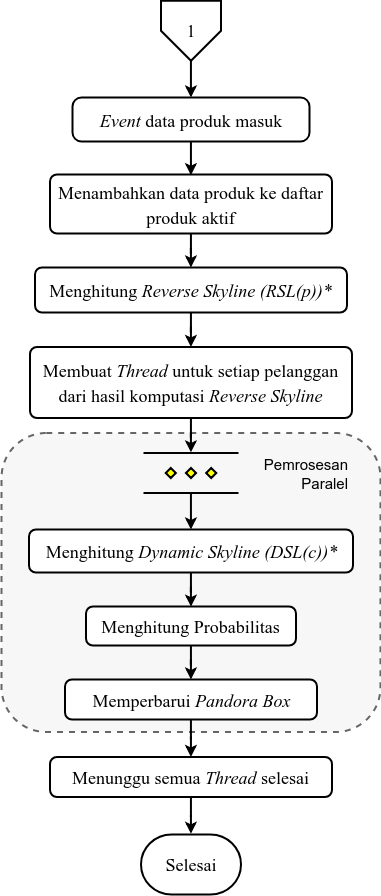
\includegraphics[width=7cm]{assets/img/bab3/flowchart-pi.png}
	\caption{Diagram Alur Proses \textit{Product Insertion}}
	\label{fig:flowchart-pi}
\end{figure}

\begin{figure}[H]
	\centering
	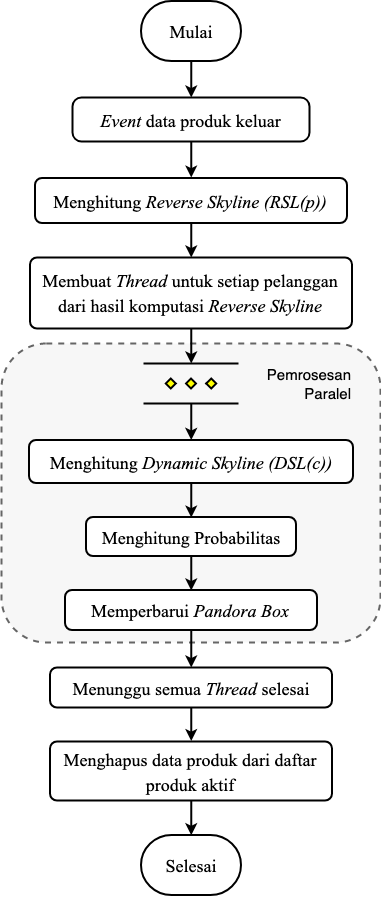
\includegraphics[width=7cm]{assets/img/bab3/flowchart-po.png}
	\caption{Diagram Alur Proses \textit{Product Deletion}}
	\label{fig:flowchart-po}
\end{figure}

\myparagraph{Proses \textit{Customer Insertion}}

Proses \textit{Customer Insertion} adalah proses yang dijalankan ketika ada data pelanggan yang masuk, dinotasikan dengan $c_{in}$. Secara garis besar, algoritme pemrosesan disajikan dalam bentuk diagram alur pada Gambar \ref{fig:flowchart-ci}. Pemrosesan diawali dengan (1) menambahkan pelanggan $c_{in}$ ke dalam daftar pelanggan aktif $C_{active}$. Kemudian (2) menghitung \textit{Initial} $DSL(c_{in})$ untuk mendapatkan hasil \textit{dynamic skyline} awal. Diakhiri dengan (3) menghitung probabilitas dan (4) memperbarui \textit{Pandora Box}.

\myparagraph{Proses \textit{Customer Deletion}}

Proses \textit{Customer Deletion} adalah proses yang dijalankan ketika ada data pelanggan yang keluar, dinotasikan dengan $c_{out}$. Secara garis besar, algoritme pemrosesan disajikan dalam bentuk diagram alur pada Gambar \ref{fig:flowchart-co}. Pemrosesan diawali dengan (1) memperbarui \textit{Pandora Box} dengan cara untuk mengisi indeks $PBox$ sebelumnya yang kosong, kemudian diakhiri dengan (2) menghapus pelanggan $c$ dari daftar pelanggan aktif $C_{active}$. 

\begin{figure}[H]
	\centering
	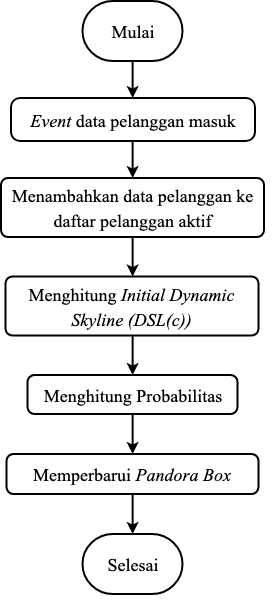
\includegraphics[width=5cm]{assets/img/bab3/flowchart-ci.png}
	\caption{Diagram Alur Proses \textit{Customer Insertion}}
	\label{fig:flowchart-ci}
\end{figure}

\begin{figure}[H]
	\centering
	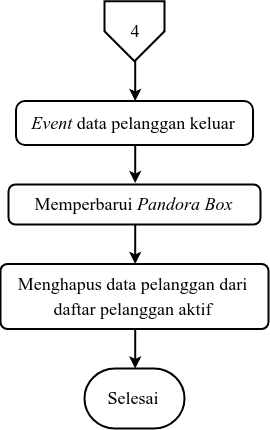
\includegraphics[width=5cm]{assets/img/bab3/flowchart-co.png}
	\caption{Diagram Alur Proses \textit{Customer Deletion}}
	\label{fig:flowchart-co}
\end{figure}

\myparagraph{Komputasi \textit{Reverse Skyline}}

Komputasi \textit{reverse skyline} digunakan untuk mencari pelanggan potensial dari sudut pandang produsen \cite{kmpp}. \textit{Reverse skyline} \cite{reverse-skyline} dari sebuah produk $p_1 \in
P$, dinotasikan dengan $RSL(p_1)$, berisi semua pelanggan $c \in C$ yang memiliki $p_1$ pada hasil \textit{dynamic skyline}-nya.

Komputasi \textit{reverse skyline} diawali dengan menentukan \textit{orthant} dari produk, dinotasikan dengan $O$. Dalam geometri, \textit{orthant} adalah analog dalam ruang data \textit{d}-dimensi atau biasa dikenal sebagai kuadran dalam bidang dua dimensi. Setiap produk $p$ memiliki $2^d$ \textit{orthant} pada data $d-$dimensi. 

\textit{Orthant} ditandai menggunakan bilangan biner. Sebagai contoh, terdapat empat \textit{orthant} pada bidang dua dimensi, yaitu $O_{00}$, $O_{01}$, $O_{10}$, dan $O_{11}$, dan delapan \textit{orthant} pada bidang tiga dimensi, yaitu $O_{000}$, $O_{001}$, $O_{010}$, $O_{011}$, $O_{100}$, $O_{101}$, $O_{110}$ dan $O_{111}$. Penggunaan bilangan biner bertujuan untuk menandai batas wilayah sebuah \textit{orthant}. Misalnya, \textit{orthant} $O_{010}$ dari produk $p_1$ memiliki wilayah dengan batas-batas sebagai berikut: sumbu $x [0:pos_x(p_1)]$, sumbu $y [pos_y(p_1):max_y]$, dan sumbu $z [0:pos_z(p_1)]$.

Langkah selanjutnya adalah menghitung \textit{midpoint} atau titik tengah antara produk kueri dan produk lainnya, misalnya $p_1$ (sebagai titik kueri) dan $p_2 \in P$, menggunakan rumus berikut: 
\begin{equation} \label{eq:midpoint2}
m_2^i = \frac{(p_1^i + p_2^i)}{2}
\end{equation}
Kemudian, menentukan \textit{midpoint skyline} atau \textit{mid-skyline} \cite{mid-skyline} pada setiap \textit{orthant}.

Langkah terakhir adalah mengecek setiap pelanggan $c \in C$ apakah didominasi oleh hasil \textit{mid-skyline} pada masing-masing \textit{orthant} atau tidak (Persamaan \ref{eq:mid-skyline}). Jika $c$ didominasi, maka $c$ tidak dapat menjadi hasil \textit{reverse skyline}.

\begin{figure}[H]
	\centering
	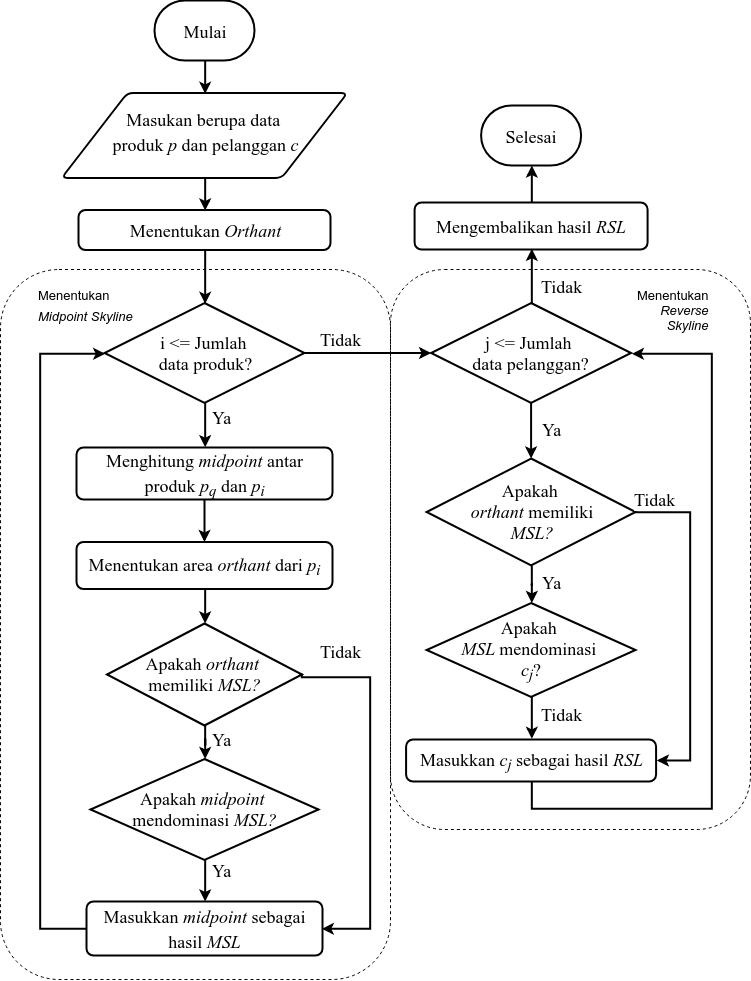
\includegraphics[width=10cm]{assets/img/bab3/flowchart-rsl.png}
	\caption{Diagram Alur Komputasi \textit{Reverse Skyline}}
	\label{fig:flowchart-rsl}
\end{figure}

\myparagraph{Komputasi \textit{Dynamic Skyline}}

Komputasi \textit{dynamic skyline} digunakan untuk mencari produk terbaik dari sudut pandang pelanggan \cite{kmpp}. \textit{Dynamic skyline} \cite{dynamic-skyline} dari seorang pelanggan $c_1 \in C$, dinotasikan dengan $DSL(c_1)$, berisi semua produk $p_1 \in P$ yang tidak didominasi oleh produk lain $p_2 \in P$ berdasarkan preferensi pelanggan $c_1$, $p_2 \nprec_{c_1} p_1$. 

Secara umum, proses komputasi \textit{dynamic skyline} diawali dengan perhitungan selisih absolut dari nilai masing-masing dimensi antara pelanggan dan produk, dinotasikan dengan:
\begin{equation}\label{eq:diff}
diff^i = |c_1^i - p^i|
\end{equation}

Selanjutnya, mengecek dominansi dinamis antar produk dengan membandingkan selisih absolut-nya. Misalnya, ada dua produk yang akan dibandingkan, dinotasikan dengan $p_s$ sebagai subjek yang dibandingkan dan $p_o$ sebagai objek pembanding. Berdasarkan syarat dominansi dinamis (Persamaan \ref{eq:syarat-dominansi-dinamis}), $p_s$ dikatakan mendominasi $p_o$ jika dan hanya jika:
\begin{equation}\label{eq:komputasi-dsl}
\begin{split}
\text{(a)} \tab diff_s^i \leq diff_o^i, \forall i \in [1, ..., d] \\
\text{(b)} \tab diff_s^i < diff_o^i, \exists i \in [1, ..., d]
\end{split}
\end{equation}

Pengecekan dominansi dinamis ini dilakukan secara iteratif sampai dipastikan suatu $p_1$ tidak didominasi oleh $p_2$ lain sama sekali. Jika $p_1$ pernah didominasi, maka $p_1$ tidak dapat menjadi hasil \textit{dynamic skyline}.

Komputasi $DSL$ dalam $k$-MPPTI dibagi menjadi 3 jenis, yaitu (1) \textit{Initial} $DSL$, digunakan ketika ada data pelanggan yang masuk, (2) $DSL-PI$, digunakan ketika ada data produk yang masuk, dan (3) $DSL-PD$, digunakan ketika ada data produk yang keluar.


\myparagraph{Perhitungan Probabilitas}

Setelah mendapatkan hasil \textit{dynamic skyline} dan \textit{reverse skyline}, selanjutnya adalah menghitung probabilitas masing-masing produk $p \in P{active}$ dipilih oleh pelanggan $c \in C{active}$ yang dinotasikan oleh persamaan berikut:
\begin{equation}\label{eq:prob-ti}
Pr_t(c, p|P_{active}) = \left\{
						\begin{array}{ll}
						\frac{1}{|DSL(c)|} & \text{if } p \in DSL(c)\\
						0 & \text{otherwise}\\
						\end{array}
						\right.
\end{equation}

Karena probabilitas produk $p$ dipilih oleh pelanggan yang tidak memiliki $p$ pada hasil \textit{dynamic skyline}-nya adalah nol, maka perhitungan probabilitas dapat disederhanakan menjadi:
\begin{equation}\label{eq:prob-ti-rsl}
Pr_t(c, p|P_{active}), \forall c \in RSL(p)
\end{equation}

\myparagraph{Perhitungan Kontribusi Pasar}

Setelah mendapatkan hasil perhitungan probabilitas, selanjutnya adalah menghitung kontribusi pasar dengan cara mengakumulasikan probabilitas produk dari setiap pelanggan $c \in Cactive$ sebagaimana yang dijelaskan pada Persamaan \ref{eq:market-contr-ti}. 
\begin{equation}\label{eq:market-contr-ti}
E_t(C, p|P_{active}) = \sum_{\forall c \in RSL(p)} Pr_t(c, p|P_{active})
\end{equation} 

\myparagraph{Pemrosesan Paralel}

Untuk meningkatkan efisiensi waktu komputasi, algoritme $k$-MPPTI mengimplementasikan konsep pemrosesan paralel, yaitu suatu bentuk komputasi dua atau lebih tugas yang dilakukan secara bersamaan dan beroperasi dengan prinsip bahwa masalah besar seringkali dapat dibagi dan dipecah menjadi masalah yang lebih kecil, kemudian dipecahkan secara bersamaan (paralel) \cite{paralel}. 

Pemrosesan paralel dilakukan dengan cara menggunakan satu atau lebih CPU atau prosesor untuk menjalankan program atau multi-\textit{thread}. Karena dilakukan secara bersamaan, maka pemrosesan ini hanya dapat dilakukan jika suatu tugas tidak membutuhkan masukan dari keluaran tugas sebelumnya, misalnya komputasi $DSL(c)$ untuk setiap $c \in RSL(p)$ yang diilustrasikan pada Gambar \ref{fig:paralel}.

\begin{figure}[h]
	\centering
	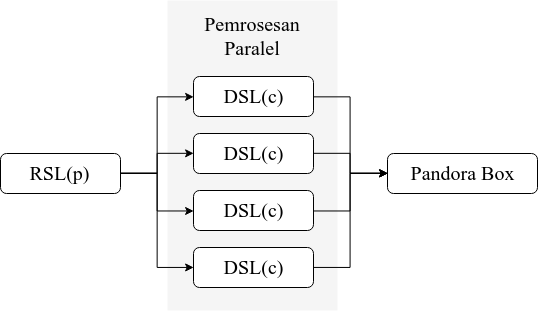
\includegraphics[width=8cm]{assets/img/bab3/paralel.png}
	\caption{Pemrosesan Paralel}
	\label{fig:paralel}
\end{figure}

\subsubsection{\textit{Query Processing}}
\tab \textit{Query processing} adalah algoritme pencarian produk sejumlah $k$ yang paling menjanjikan dalam interval waktu tertentu. Selanjutnya kueri ini disebut dengan $k$-MPPTI ($k$-\textit{Most Promising Products in Time Interval}) yang dinotasikan oleh Persamaan \ref{eq:kmppti}. 
\begin{equation}\label{eq:kmppti}
k-MPPTI(k, [t_i:t_e])
\end{equation} 

Kueri $k$-MPPTI hanya membutuhkan dua masukan saja, yaitu bilangan bulat positif $k$ yang lebih kecil dari $|P|$ sebagai jumlah produk yang dicari dan interval waktu pencarian yang terdiri dari waktu awal dan waktu akhir $[t_i:t_e]$. Berbeda dengan kueri $k$-MPP (Persamaan \ref{eq:kmpp}), kueri $k$-MPPTI tidak membutuhkan masukan \textit{dataset} produk $P$ dan preferensi pelanggan $C$ lagi karena sudah melalui tahap \textit{data precomputing} yang menghasilkan \textit{Pandora Box}.  

Algoritme ini mengadopsi strategi pemilihan produk $k$-MPP, yaitu memilih \textit{subset} $k$ produk $P'$ dari $P$ yang memiliki kontribusi pasar lebih besar dibandingkan dengan \textit{subset} $k$ produk $P''$ dari $P$ yang lain \cite{kmpp}. Bedanya, $k$-MPPTI menambahkan fitur pembatasan interval waktu pencarian.

\begin{figure}[h]
	\centering
	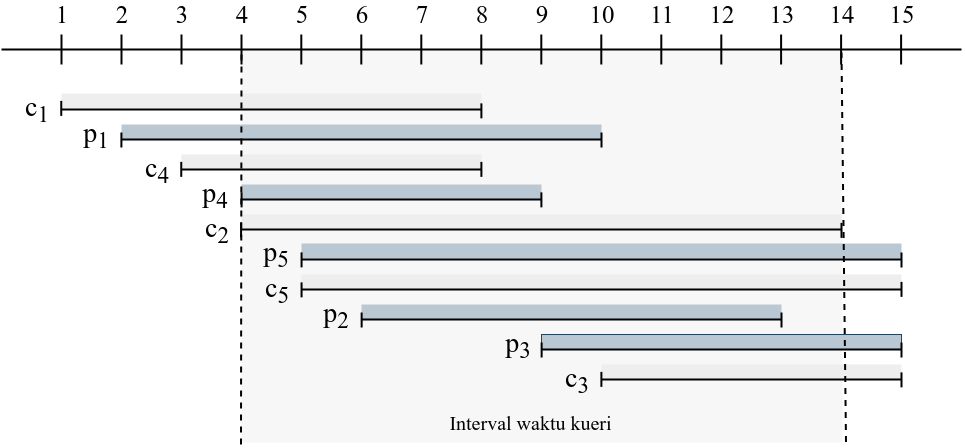
\includegraphics[width=10cm]{assets/img/bab3/timeline-interval.png}
	\caption{Ilustrasi Interval Waktu Pencarian}
	\label{fig:timeline-kueri}
\end{figure}

Ada dua langkah pemrosesan yang harus dilakukan, yaitu (1) mengakumulasi skor kontribusi pasar setiap produk $p \in P$ dalam interval waktu pencarian. Total kontribusi pasar berbasis interval waktu dinotasikan sebagai $MC_{[t_i:t_e]}(p), \forall p \in P$. Kemudian (2) mengurutkan total skor dari yang terbesar dan mengembalikan produk sejumlah $k$ teratas sebagai hasil dari kueri pencarian. 

Misalnya, seorang pengguna ingin mencari $3$ produk yang paling menjanjikan dalam interval waktu $4$ hingga $14$, dinotasikan dengan $k-MPPTI(3, [4:14])$. Berdasarkan hasil perhitungan total kontribusi pasar berbasis interval waktu pada Tabel \ref{tab:mc-ti-res}, produk $p_5$, $p_2$ dan $p_4$ adalah $3$ produk paling menjanjikan dalam interval waktu $4$ hingga $14$.

\begin{figure}[h]
	\centering
	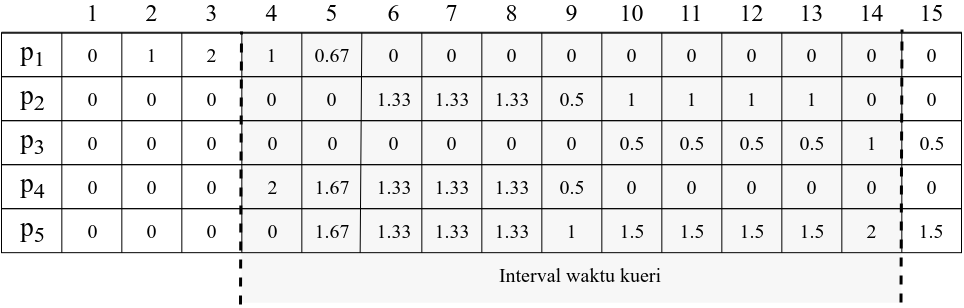
\includegraphics[width=10cm]{assets/img/bab3/pbox-kueri.png}
	\caption{Perhitungan Kontribusi Pasar pada \textit{Pandora Box} Berdasarkan Interval Waktu Pencarian}
	\label{fig:pbox-kueri}
\end{figure}

\begin{table}[H]
	\small
	\centering
	\begin{tabular}{|p{3cm}|p{2cm}|}
		\hline
		$MC_{[4:14]}(p_5)$ & $14.67$ \\ \hline
		$MC_{[4:14]}(p_2)$ & $8.5$ \\ \hline
		$MC_{[4:14]}(p_4)$ & $8.17$ \\ \hline
		$MC_{[4:14]}(p_3)$ & $3$ \\ \hline
		$MC_{[4:14]}(p_1)$ & $1.67$ \\ \hline
	\end{tabular} 
	\caption{Hasil Perhitungan Kontribusi Pasar Berbasis Interval Waktu}
	\label{tab:mc-ti-res}
\end{table}

Interval waktu pencarian sangat mempengaruhi hasil kueri. Sebagai bukti, jika interval waktu pencariannya diubah dari $1$ hingga $6$, $[1:6]$, maka hasil kueri $3$ produk teratas yang paling menjanjikan adalah $p_4$, $p_1$, dan $p_5$.

\begin{table}[H]
	\small
	\centering
	\begin{tabular}{|p{3cm}|p{2cm}|}
		\hline
		$MC_{[1:6]}(p_4)$ & $5$ \\ \hline
		$MC_{[1:6]}(p_1)$ & $4.67$ \\ \hline
		$MC_{[1:6]}(p_5)$ & $3$ \\ \hline
		$MC_{[1:6]}(p_2)$ & $1.33$ \\ \hline
		$MC_{[1:6]}(p_3)$ & $0$ \\ \hline
	\end{tabular} 
	\caption{Hasil Perhitungan Kontribusi Pasar Berbasis Interval Waktu (2)}
	\label{tab:mc-ti-res2}
\end{table}


\subsection{Algoritme \textit{Brute Force}}
\tab Algoritme \textit{brute force} adalah algoritme yang mengimplementasikan metode \textit{brute force}, yaitu melakukan percobaan terhadap semua kemungkinan dan hanya mengandalkan kekuatan pemrosesan komputer. Algoritme ini digunakan sebagai pembanding dari algoritme $k$-MPPTI.

Secara garis besar, struktur data dan pendekatan yang digunakan hampir sama dengan $k$-MPPTI, namun tidak ada tahap komputasi $RSL$, sehingga komputasi $DSL$ dilakukan pada semua $c \in C$ dengah cara membandingkan semua produk $p \in P$ satu persatu. Selain itu, komputasi tidak dilakukan dengan secara paralel. 

\subsection{Arsitektur Aplikasi} 
\tab Sistem akan diimplementasikan menggunakan arsitektur \textit{client}-\textit{server} seperti yang diilustrasikan pada Gambar \ref{fig:arsitektur}. Terdapat dua komponen utama dalam arsitektur ini, yaitu klien (\textit{client}), pihak yang meminta atau menerima layanan, dan peladen (\textit{server}), pihak yang memberikan atau mengirim layanan. Komponen-komponen ini terhubung ke jaringan, baik melalui kabel maupun nirkabel untuk melakukan transmisi data. 

\begin{figure}[h]
	\centering
	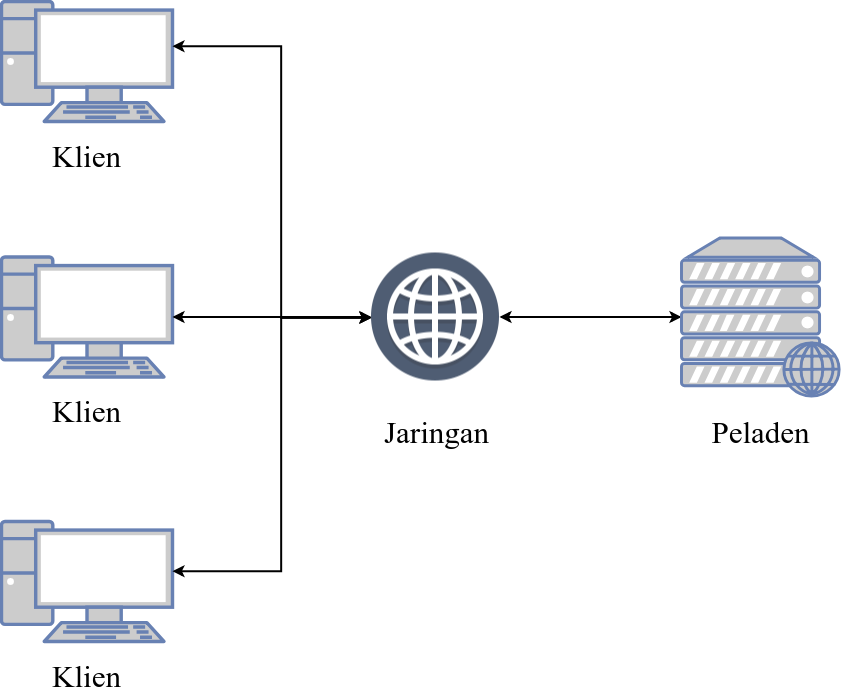
\includegraphics[width=7cm]{assets/img/bab3/arsitektur.png}
	\caption{Perancangan Arsitektur Aplikasi}
	\label{fig:arsitektur}
\end{figure}

Klien mengimplementasikan antarmuka pengguna grafis atau APG (Inggris: \textit{graphical user interface} atau GUI) berbasis web, sedangkan peladen mengimplementasikan \textit{back-end service} yang berisi algoritme komputasi $k$-MPPTI yang terdiri atas algoritme \textit{data precomputing} dan \textit{query processing}. Web dibangun menggunakan Flask \textit{microframework} dan bahasa Python, HTML, CSS, serta Javascript, sedangkan \textit{back-end service} diimplementasikan menggunakan bahasa Python. Flask juga sekaligus berperan sebagai peladen web (\textit{web server}).

Pengguna melakukan masukan data melalui web, kemudian data tersebut dikirimkan ke \textit{back-end service} untuk dilakukan proses \textit{data precomputing}. Setelah hasil \textit{data precomputing} selesai, pengguna melakukan masukan kueri pencarian. Kueri pencarian tersebut akan dikirimkan ke \textit{back-end service} untuk dilakukan proses \textit{query processing}. Hasil yang didapatkan akan dikembalikan ke klien, disertai dengan visualisasi data.
